\chapter{Použité technologie}
\label{ch:technology}
V této kapitole se budu věnovat popisu technologii, které jsem použil při vývoji rozhraní nebo jsem mezi nimi uvažoval. V první části se zaměřím na programovací jazyky, které jsou hlavní kamenem pro volbu správného frameworku. Od použití frameworku se již odvíjí další technologie spadající do kategorie frontendu a backendu. Jako poslední budu popisovat technologie, které se užívají v běžném vývoji webových aplikací.

\section{Programovací Jazyky}
\label{sec:languages}
Programovací jazyky v kontextu uživatelského rozhraní (UI) hrají klíčovou roli ve vývoji a implementaci interaktivních prvků. Zaměřím se tak především na jazyky, které jsem použil a které jsou nejčastěji využívány v rámci vývoje webových aplikací, jejich výhody a nevýhody a jakým způsobem se liší od sebe.

\subsection{Kompilované Jazyky}
\label{subsec:languages-compiled}
Mezi první druh programovacích jazyků patří jazyky kompilované, které se při jejich zpracování převádí přímo na kód strojový. Tento proces se nazývá kompilace a výsledný kód je následně spustitelný na konkrétním operačním systému. Tento způsob zpracování má několik výhod:

\begin{itemize}
    \item \textbf{Rychlost:} Kód, který již byl jednou přeložen, je okamžitě spustitelný bez dalšího zpracování.
    \item \textbf{Výkon:} Díky překladu do strojového kódu, je možné při kompilaci provádět optimalizace, které zvyšují výkon aplikace.
    \item \textbf{Bezpečnost:} Kompilované jazyky ošetřují mnoho chyb již při jejich kompilaci, což zvyšuje bezpečnost aplikace a snižuje rizika chyb.
\end{itemize}

Mezi nejznámější kompilované jazyky můžeme zařadit jazyky jako C, C++, Java, Rust, Go a mnoho dalších. V rámci této práce jsem se zaměřil na jazyk \textit{TypeScript} a \textit{Less}, který mi tak usnadní vývoj frontendu aplikace.

\subsubsection{TypeScript}
\label{subsubsec:languages-compiled-typescript}
TypeScript je jedním z kompilovaných jazyků, který byl vytvořen jako nadstavba nad existující jazyk \textit{JavaScript}. Poprvé bych uveden v roce 2012 společností Microsoft a jeho hlavním cílem je obohacení JavaScriptu o statické typování, které umožňuje programátorům definovat typy proměnných, parametrů funkci a návratových hodnot. Mimo statické typování dále obohacuje JavaScript o funkce jako jsou třídy, moduly, generické typy a další. Díky těmto funkcím je možné zabezpečit kód proti chybám, které by mohli vzniknout v průběhu vývoje aplikace pod standardním JavaScriptem.

Oproti jiným jazykům sám o sobě není spustitelný, ale je nutné jej nejprvě přeložit do kódu JavaScriptu, Tento proces se nazývá transpilace pomocí nástroje \textit{tsc}, který je součástí balíčku \textit{Node.js}.

\subsubsection{Less}
\label{subsubsec:languages-compiled-less}
Less je dalším z kompilovaných jazyků, které se zaměřují na zlepšení a obohacení jazyka \textit{CSS}. Tento jazyk byl vytvořen v roce 2009 autorem Alexis Sellier a jako TypeScript je jeho cílem poskytnout dodatečné funkce pro pohodlnější a efektivnější psaní kaskádových stylů. Jako hlavní výhody můžeme uvést možnost definovat proměnné, funkce nebo vnořování selectoru.

Pro využití Less je nutné jej přeložit do kódu CSS, což je možné provést pomocí nástrojů jako jsou \textit{Less.js} nebo \textit{Node.js}.

\subsection{Interpretované Jazyky}
\label{subsec:languages-interpreted}
\textcolor{red}{DOPLNIT - Co je to interpretovaný jazyk, jaké má výhody a nevýhody, jaké jazyky jsou interpretované}

\subsubsection{JavaScript}
\label{subsubsec:languages-interpreted-javascript}
\textcolor{red}{DOPLNIT - Co je to JavaScript, jaké má výhody a nevýhody, jaké jazyky jsou interpretované}

\subsubsection{Python}
\label{subsubsec:languages-interpreted-python}
\textcolor{red}{DOPLNIT - Co je to Python, jaké má výhody a nevýhody, jaké jazyky jsou interpretované}

\subsection{Značkovací Jazyky}
\label{subsec:languages-markup}
\textcolor{red}{DOPLNIT - Co je to značkovací jazyk, jaké má výhody a nevýhody, jaké jazyky jsou značkovací}

\subsubsection{HTML}
\label{subsubsec:languages-markup-html}
\textcolor{red}{DOPLNIT - Co je to HTML, jaké má výhody a nevýhody, jaké jazyky jsou značkovací}

\subsubsection{Markdown}
\label{subsubsec:languages-markup-markdown}
\textcolor{red}{DOPLNIT - Co je to Markdown, jaké má výhody a nevýhody, jaké jazyky jsou značkovací}

\section{Frameworky}
\label{sec:dev-framework}
Framework, v jiných slovech struktura nebo kostra, představuje v informatice a softwarovém inženýrství abstraktní koncept poskytující základní stavební kameny pro aplikace s širokým spektrem funkcí. Cílem frameworků je usnadnit vývoj aplikací tím, že nabízejí předem definovanou strukturu, kterou lze dále rozšiřovat o vlastní kód a funkcionalitu. Tímto způsobem umožňují frameworky vývojářům rychleji a efektivněji vytvářet aplikace, což přináší zvýšení produktivity, snížení nákladů na vývoj a hlavně standardizaci kódu mezi vývojáři.

Ve svéře informatiky se frameworky dělí podle programovacího jazyku nebo zaměření na aplikace. Máme zde druhy frameworku určených na vývoj webů, her, mobilních aplikací nebo čistě na široký výzkum. \cite{about_framework}

\subsection*{Rozdíl mezi Frameworkem a Knihovnou}
Framework a knihovna jsou dvě často zaměňované koncepce, avšak existují zásadní rozdíly mezi nimi. Knihovna je soubor funkcí nebo tříd, které lze využít při vytváření aplikace. Zajišťuje určitou funkcionalitu, ale vývojář nese odpovědnost za řízení toku aplikace a volání funkcí knihovny.

Naopak framework poskytuje kompletní strukturu aplikace, kde vývojář implementuje pouze specifickou funkcionalitu. Framework tak aktivně řídí tok aplikace a volá konkrétní části kódu, zatímco vývojář se zaměřuje na přizpůsobení těchto specifických částí.

\begin{figure}[H]
    \centering
    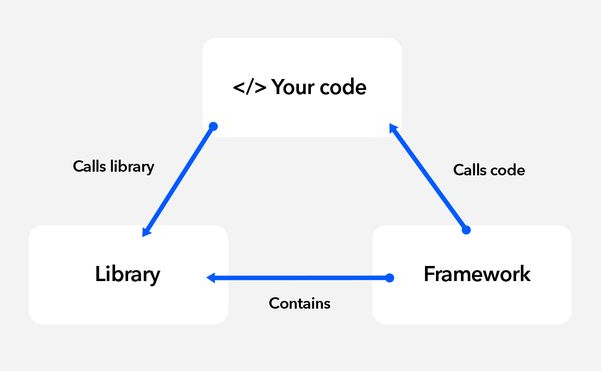
\includegraphics[width=0.6\textwidth]{figures/framework_library_difference}
    \caption{Rozdíl mezi \textit{Frameworkem} a \textit{Knihovnou}. \cite{framework_library_difference}}
    \label{fig:framework_library_difference}
\end{figure}

\subsection*{Model-View-Template vs. Model-View-Controller}
Model-View-Template dále jen jako MVT a Model-View-Controller dále jen jako MVC jsou návrhové vzory, které se široce využívají v softwarovém vývoji webových aplikací. Tyto vzory rozdělují průběh aplikaci do tří propojených částí, kde každá část má svou specifickou roli a odpovědnost. Díky této struktuře je možné izolovat různé části aplikace a tím zvyšovat modularitu, znovu použitelnost a udržitelnost kódu.

V případě MVT je aplikace rozdělena na tři části: \textit{Model}, \textit{View} a \textit{Template}. Model zde reprezentuje datovou strukturu, většinou tedy namapované objekty získané z databáze, případně z jiného zdroje. View (zobrazení) je zodpovědné za přijímání uživatelských požadavků a zobrazování odpovědi od serveru zpět uživateli, v rámci této komunikace reprezentuje určitý most mezi modelem a šablonou. Jako poslední je zde template (šablona), která v tomto případě přijatá data zpracovává do výsledného HTML kódu pomocí speciálních značek určující předem daný formát stránky. Výsledný HTML kód je následně odeslán zpět uživateli.

Na druhé straně MVC, který je často používán ve zbytku frameworku se oproti MVT liší pouze lehce. Model zde stále reprezentuje datovou strukturu, ale View je naopak zodpovědný o pouhé vykreslování dat uživateli. Novým prvkem je zde Controller, který se zaobírá zbylou interakcí uživatele s aplikací, tedy přijímání požadavků, zpracování dat a následné odeslání zpět uživateli. \cite{mvc_mvt_difference}

\begin{figure}[H]
    \centering
    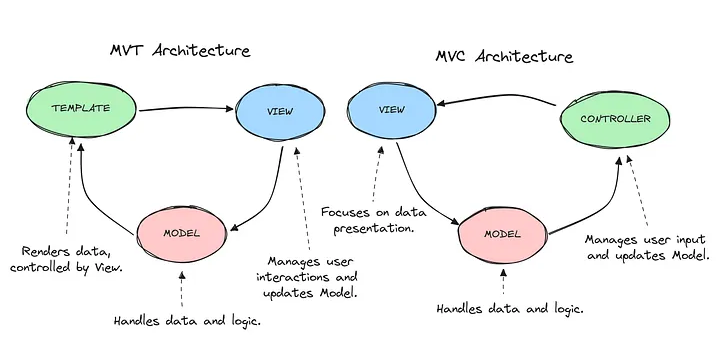
\includegraphics[width=1.0\textwidth]{figures/mvc_mvt_difference}
    \caption{Rozdíl mezi \textit{Model View Template} a \textit{Model View Controller} návrhovými vzory. \cite{mvc_mvt_difference_img}}
    \label{fig:mvc_mvt_difference}
\end{figure}

\subsection{Django}
\label{subsec:dev-framework-django}
Django je výkonným open-source frameworkem určeným pro vývoj robustních a lehce škálovatelných webových aplikací v programovacím jazyce Python. Od svého veřejného uvedení v roce 2005, pojmenovaného po slavném kytaristovi Django Reinhardtovi, získal popularitu díky své schopnosti urychlit vývoj a poskytnout bezpečné a efektivní nástroje pro tvorbu webových aplikací.

Framework Django přistupuje k architektuře webových aplikací pomocí návrhového vzoru Model-View-Template (MVT), což představuje alternativu k tradičnímu přístupu Model-View-Controller (MVC). Tato struktura usnadňuje komunikaci mezi datovým modelem, prezentační vrstvou a šablonami pro serverové vykreslování.

V oblasti vývoje uživatelského rozhraní Django nabízí šablonovací jazyk (DTL), který umožňuje vytvářet dynamická a daty řízená uživatelská rozhraní. To je zvláště užitečné pro aplikace, které kladou důraz na optimalizaci pro vyhledávače (SEO) a vyžadují komplexní logiku na straně serveru. DTL umožňuje vývojářům vytvářet stránky s dynamickým obsahem, který je generován ještě před odesláním HTML kódu ze serveru.

V situacích, kde je potřeba dosáhnout interaktivity uživatele s rozhraním, je možné rozšířit Django o JavaScriptové knihovny nebo volit jiný framework specializovaný na frontendový vývoj. To umožňuje vysoce flexibilní přístup k vytváření moderních a interaktivních webových aplikací. \cite{about_django}.

\subsection{React}
\label{subsec:dev-framework-react}
React je významná JavaScriptová knihovna určená pro vytváření uživatelských rozhraní, především na straně klienta. Vyvinutá firmou Facebook, React využívá virtuální DOM k efektivní aktualizaci komponent a podporuje deklarativní syntaxi pro tvorbu interaktivních uživatelských rozhraní. Je široce používán pro vývoj jednostránkových aplikací (SPA), kde je klíčová potřeba dynamických aktualizací.

React vyniká v poskytování responzivního a interaktivního uživatelského přístupu, což z něj činí oblíbenou volbu pro moderní webový vývoj. Jeho komponentový přístup umožňuje rozdělit uživatelské rozhraní do znovupoužitelných částí, což zjednodušuje správu a údržbu kódu. Využívá návrhový vzor \textit{Model-View-Controller}. \cite{about_react}

\subsection{Angular}
\label{subsec:dev-framework-angular}
Angular je populární open-source framework pro vývoj webových aplikací. Je sponzorován a udržován převážně společností Google a vyniká díky široké komunitě a schopnosti řešit výzvy spojené s vývojem jednostránkových aplikací (SPA). Angular je postaven na jazyce TypeScript a využívá komponentovou architekturu pro tvorbu uživatelských rozhraní.

Jednou z klíčových vlastností Angularu je jeho komplexní systém modulů a komponent, který usnadňuje organizaci a správu kódu. Angular používá návrhový vzor \textit{Model-View-Controller} (MVC) a klade důraz na dvoucestný data-binding, což znamená, že změny v modelu automaticky odrážejí změny v vykreslování a naopak.

Framework obsahuje mnoho vestavěných funkcí, jako například modulární routování, HTTP služby pro komunikaci se serverem, a nástroje pro testování. Angular také poskytuje kompletní sadu nástrojů pro správu stavu aplikace. \cite{about_angular}

\subsection{Laravel}
\label{subsec:dev-framework-laravel}
Laravel je moderní open-source PHP framework, který je určený pro vývoj webových aplikací. Tento framework vytvořil Taylor Otwell a byl poprvé vydán v roce 2011. Vyniká díky své jednoduchosti, efektivitě a schopnosti urychlit vývoj aplikací. Laravel využívá návrhový vzor \textit{Model-View-Controller} (MVC) a poskytuje mnoho vestavěných funkcí, jako například routování, šablonovací systém, a nástroje pro správu databáze.

Mezi jednu z jeho klíčových vlastností patří Eloquent ORM, což je moderní implementace Active Record návrhového vzoru, který umožnuje jednoduše pracovat s namapovanými objekty z databáze jako s obyčejnými PHP objekty. Jako framework Django obsahuje šablonovací systém Blade, které je jednoduchý a efektivní pro vytváření dynamických uživatelských rozhraní. Další výhodou jsou zabudované mechanismy pro zabezpečení aplikace, jako například ochrana proti Cross-Site Scripting (XSS) a SQL Injection útokům. \cite{about_laravel}

\subsection{Vue.js}
\label{subsec:dev-framework-vuejs}
Vue.js je moderní JavaScriptový framework určený pro vývoj uživatelského rozhraní webových aplikací. Jeho největší výhodou je snadná flexibilita a jednoduchá intergrace s již existujícími projekty. Vue.js byl poprvé vydán v roce 2014 a od této doby získal velkou popularitu díky své schopnosti urychlit vývoj a poskytnout efektivní nástroje pro tvorbu moderních webových aplikací.

Jedním z klíčových prvků Vue.js je reaktivní datová vrstva, která umožňuje snadná sledování a aktualizaci dat. Framework využívá jednosměrný datový tok, což znamená, že veškeré změny v datech jsou automaticky aktualizovány v uživatelským rozhraní. Toto chování usnadňuje sledování stavu aplikace a vytváření dynamických a interaktivních uživatelských rozhraní.

Vue.js je navržen ohledem na progresivitu, což znamená, že ho lze snadno a postupně intergrovat do existujícího projektu a nijak tak nenarušit jakoukoliv funkčnost. Při této integraci lze jednoduše rozdělit aplikaci do Frontend části, reprezentovanou Vue.js a backend části, která může být reprezentována například frameworkem Django. \cite{about_vuejs}

\subsection{Svelte}
\label{subsec:dev-framework-svelte}
Svelte je jedním z inovativních JavaScriptových frameworků, který se zaměřuje na efektivní kompilací v ranné fázi build procesu, což přináší nový pohled na vývoj uživatelské rozhraní. Zatímco tradiční frameworky provadějí většinu práce na straně klienta nebo serveru za běhu, Svelte přesouvá tuto činnost do fáze komiplace, čímž mnohonásobně zlepšuje výkon a optimalizuje výslednou velikost kódu.

Klíčovým konceptem Svelte je štěpení kódu do komponent, které jsou více než pouze části uživatelské rozhraní. Tyto komponenty obsahuje více než prezentační logiku, definují také jak se má komponent chovat a jaké akce má provádět pod určitými podmínkami. Tento přístup tak umožnuje jednoduše eliminovat zbytečný nebo duplicitní kód ve fázi kompilace, jako dělají například \textit{C++ kompilátory}.

Pro plné využití tohoto frameworku, je nutné jeho rozšíření o backendovou část, která bývá zodpovědná za zpracování dat a komunikaci se serverem. Tato část může být reprezentována například jedním s frameworků zmíněných výše. \cite{about_svelte}

\subsection{Shrnutí a Srovnání}
\label{subsec:dev-framework-comparison}
Srovnání frameworku zmíněných výše dosahuje celkového závěru, že každý z ních má své výhody a nevýhody. Pomocí každého frameworku nebo jejich kombinací lze vytvořit moderní a efektivní webové aplikace, které by splňovaly mnoho požadavků ze strany efektivního vývoje, výkonu a bezpečnosti.
Každý z frameworků používá jiný jazyk, ať to je buď Python, JavaScript nebo PHP, což může být klíčové pro jeho výběr vzhledem k projektu. Dalším faktorem je dokumentace, komunita a dostupnost nástrojů, které mohou zajistit rychlý vývoj a řešení problémů.

Pro můj projekt jsem nakonec zvolil \textbf{Django}. Tento framework jsem zvolil z důvodu, že jsem s ním již v minulosti pracoval a mám tedy určité znalosti a schopnosti pracovat pod jazykem Python. Pokud se podíváme na srovnání frameworku, Django není moc populárním v oblasti frontendu, ale díky jeho šablonovacímu systému a možností rozšíření o JavaScriptové knihovny lze tyto nedostatky vykompenzovat.

\begin{figure}[H]
    \centering
    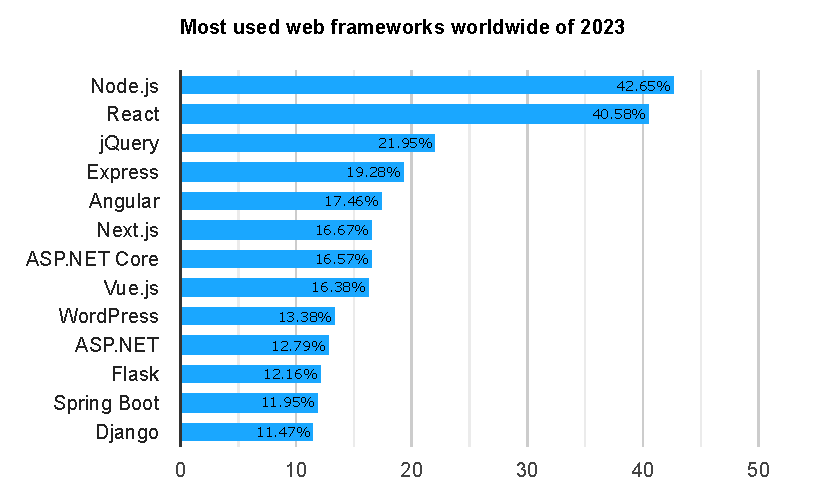
\includegraphics{figures/frameworkGraphs}
    \caption{Srovnání webových frameworku pro rok 2023. \cite{framework_comparison}}
    \label{fig:framework_comparison}
\end{figure}

\section{Zpracování požadavku}
\label{sec:dev-request-processing}
Zpracování požadavku je klíčovým prvkem webových aplikací, vzhledem k rozsáhlým rozdílům u frameworku je nutné si blíže představit jak takové zpracování probíhá. V rámci tohoto procesu se setkáváme s dvěma typy zpracování \textit{Server-Side} a \textit{Client-Side}. Jako třetí druh zpracování se dá považovat i \textit{Hybridní} neboli \textit{Pre-Rendering}, který kombinuje oba přístupy.

Při vývoji je nutné si předem určit, který ze stylů zpracování bude pro projekt použit, přechod mezi jednotlivými druhy již v průběhu vývoje může být velmi zdlouhavý a finančně náročný. \cite{request_processing}

\subsection{Server-Side Rendering}
\label{subsec:dev-request-processing-server-side-rendering}
Server-Side Rendering (SSR) je často využívaný způsob zpracování, který se obvykle uplatňuje u menších webových aplikací, jež bývají označovány jako statické stránky. Tyto stránky svůj obsah po zpracování již nikdy nemění. Základem SSR je, že veškeré zpracování dat probíhá na straně serveru, a klient poté již obdrží kompletně vykreslenou stránku, kterou prohlížeč jednoduše načte. Tyto stránky díky své statické povaze dosahuji často vysokých hodnocení v SEO, což je klíčové pro zvýšení návštěvnosti.

Jednou z nevýhod SSR je však vysoká náročnost na vypočetní výkon serveru. Tento problém se projevuje zejména v případě, kdy server zaznamená velké množství klientských požadavků v krátkém časovém období. Při každém požadavku dojde k novému kompletnímu vykreslení stránky, i když se obsah stránky změnil jen minimálně.

\begin{figure}[H]
    \centering
    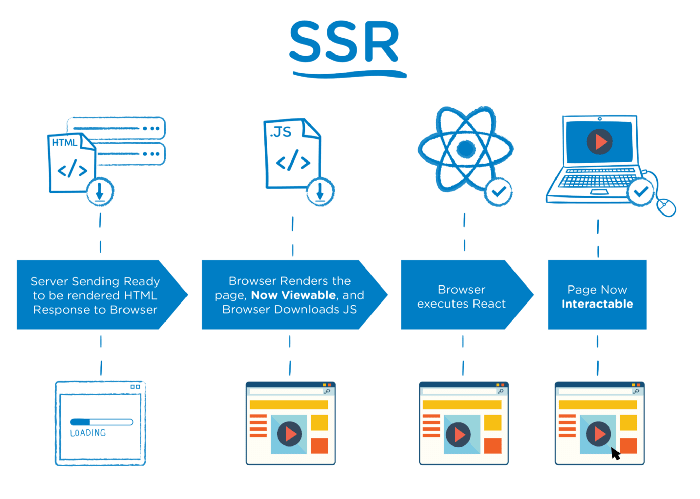
\includegraphics[width=1.0\textwidth]{figures/server-side-rendering}
    \caption{Postup Server-Side renderingu při žádosti o stránku. \cite{rendering-diff}}
    \label{fig:server-side-rendering}
\end{figure}

\subsection{Client-Side Rendering}
\label{subsec:dev-request-processing-client-side-rendering}
Client-Side Rendering (CSR) je moderní způsob zpracování webových stránek, jehož využití se rozšířilo s příchodem programovacího jazyka JavaScript do světa World-Wide-Web (WWW). Tento přístup umožňuje dynamické vykreslování obsahu stránek přímo na straně klienta, což výrazně snižuje zátěž serveru a zvyšuje rychlost zpracování požadavků.

Ve srovnání s Server-Side Renderingem (SSR) je u CSR náročnější dosáhnout vysokého skóre v oblasti SEO. Důvodem je, že proces vykreslování stránky u klienta může trvat proměnlivě dlouho a existují rizika, že webcrawler, který indexuje stránku ji opustí ještě před jejím kompletním načtením. Tento problém lze řešit pomocí techniky \textit{Pre-Rendering}, kterou popisuji v následující sekci.

\begin{figure}[H]
    \centering
    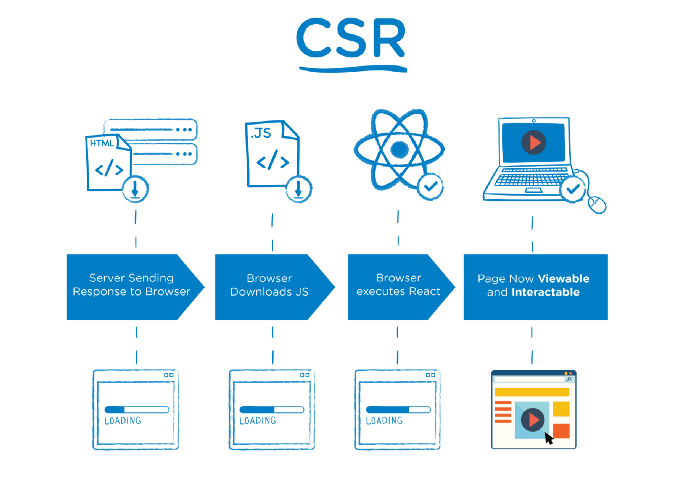
\includegraphics[width=1.0\textwidth]{figures/client-side-rendering}
    \caption{Postup Client-Side renderingu při žádosti o stránku. \cite{rendering-diff}}
    \label{fig:client-side-rendering}
\end{figure}

\subsection{Hybrid Rendering}
\label{subsec:dev-request-processing-hybrid-rendering}
Hybrid Rendering, také známy jako Pre-Rendering, představuje moderní přístup k zpracování webových stránek, který se pokouší o skloubení výhod Server-Side a Client-Sider renderingu. Tento přístup jednoduše umožnuje vývojářům vytvářet takhzvané \("\)skeleton\("\) stránky, které jsou odeslány klientovi ihned po přijetí požadavku. Po následném načtení stránky klientem, dochází k dynamickému vykreslení obsahu, kde dojde k nahrazení pouze daných části webu, které obsahovaly dynamický obsah.

\section{Technologie}
\label{sec:dev-technology}
V nynější sekci se zaměřím na popis bližší popis technologii, které lze využívat během vývoj nebo přímo v rámci daného frameworku. Mezi tyto technologie spadá široké spektrum nástrojů, knihoven, jazyký a dalších prvků, které jsou volně dostupné na internetu a mají za cíl usnadnit vývoj a zvýšit efektivitu vývojáře.

\subsection{Šablonování}
\label{subsec:dev-technology-templating}
Šablonování je klíčovou technologií v rámci vývoje webových aplikací, která slouží k oddělení prezentace dat od logiky jejich zpracování. Tento přístup umožňuje vývojářům a designérům efektivně spolupracovat na vytváření jak statických tak dynamických uživatelských rozhraní, zatímco zvyšuje modularitu, udržitelnost a bezpečnost kódu. Šablonování se většinou využívalo jako externí knihovna, ale s příchodem moderních frameworků jako je Django, React nebo Angular, se stalo nedílnou součástí těchto frameworků.

Jako systém umožňuje definovat strukturu a vzhled webových stránek pomocí šablon, které se na sebe mohou vázat nebo se rozšiřovat. Každá z těchto šablon obsahuje statický HTML kód spolu s vloženými proměnnými, filtry a řídícími strukturami. Finální šablony se poté před odesláním klientovi zpracují na serveru, a výsledný HTML kód je odeslán klientovi.

Mezi hlavní výhody používání šablon patří:
\begin{enumerate}
    \item \textbf{Oddělení Prezentace a Logiky:} Šablonovací systém oddělením prezentace dat a logiky zpracování umožňuje vývojářům a designérům efektivně spolupracovat.
    \item \textbf{Univerzální Použitelnost:} Šablony lze použít pro vytváření jak statických tak dynamických uživatelských rozhraní, což zvyšuje modularitu a znovupoužitelnost kódu.
    \item \textbf{Podpora Dynamických Dat:} Díky použití proměnných a filtrů umožňuje šablonovací systém dynamicky zobrazovat data na stránkách. To je klíčové pro vytváření interaktivních a daty řízených uživatelských rozhraní.
    \item \textbf{Zabezpečení:} Systém frameworku obsahuje mechanismy pro prevenci útoků jako Cross-Site Scripting (XSS), Form tampering, SQL injection a další. Tato zabezpečení jsou automaticky aplikována na šablony, což zvyšuje bezpečnost aplikace.
\end{enumerate}

Celkově lze konstatovat, že technologie šablonování přispívá k efektivnímu a strukturovanému vývoji webových aplikací, usnadňuje spolupráci mezi vývojáři a designéry a zvyšuje obecnou robustnost aplikace. Pro svůj projekt jsem zvolil šablonovací systém \textbf{Django Template Language (DTL)}, který je součástí frameworku Django.

\lstinputlisting[language=HTML, caption={Příklad použití templatu v Djangu.}, label={lst:django-template-example}]{sourceCodes/DjangoTemplateExample.html}

Na výše uvedeném zdrojovém kódu lze vidět několik \textit{block} značek, které rozdělují šablonu na jednotlivé části. Tyto bloky lze pak následně později implementovat v jiných šablonách kde se daná šablona rozšiřuje. Na řádku 19. tak můžeme vidět, že sekce \textit{content} bude později implementována.

\subsection{Boostrap}
\label{subsec:dev-technology-bootstrap}
Bootstrap je open-source framework, který byl původně vytvořen firmou Twitter s hlavním cílem zjednodušit vývoj konzistentních a responzivních uživatelských rozhraní pro webové aplikace a stránky. Tento framework se tak stal díky jeho modularitě a flexibilitě jedním z nejpopulárnějších nástrojů pro vývojáře a designéry.

Jeho klíčovou vlastní, která přímo navazuje na principy responzivního designu~\ref{subsec:ui-gui-theory-responsive-design} zmíněné v předchozí sekci, je použití tzv. \textit{Grid systému}, tedy rozložení mřížky. Tento systém Boostrapu tak umožňuje vývojářům snadno vytvářet komplexní rozložení stránek za použití základních předdefinovaných tříd, které určují šířku sloupců, vnitří a vnější okraje a další. Při změně velikosti obrazovky pak dojde v systému o automatické přizpůsobení velikosti jednotlivých oken čímž nevzniknou žádné problémy s rozložením komponent.

Bootstrap nadále neobsahuje pouze předdefinovaný CSS třídy, ale obsahuje také nemalé množství JavaScriptových pluginů, které tak rozšiřuj funkčnost základních komponent HTML o interaktivitu. Příkladem takové komponenty může být například \textit{Dropdown}, \textit{Modal}, \textit{Carousel} a další.

V praxi tak lze tento systém velmi snadno implementovat do jakéhokoliv projektu. Pro jeho implementaci stačí přidat odkazy na soubory CSS a JavaScript do hlavní HTML dokumentu, po správném vložení tak lze ihned začít využívat komponent Bootstrapu. Díky této praktiky tak je možné urychlit vývoj prototypů aniž by bylo nutné psát vlastní styly.

\endinput